\noindent
\begin{tabular}{cc}
\begin{minipage}{0.95\textwidth}
\begin{exerciseS}[Galleria a circuito aperto]
 Viene chiesto di determinare la potenza dei motori della galleria a circuito aperto rappresentata in figura, sapendo che la velocità massima desiderata nella sezione di prova è $V_{test} = 30 \, m/s$, l'area della sezione di prova è $A_{test} = 1.0 \, m^2$ e l'area della sezione in cui è alloggiato il ventilatore che mette in moto l'aria è $A_{fan} = 2.0 \, m^2$. Si supponga che la corrente sia incomprimibile e che la densità dell'aria sia $\rho = 1.1 \, kg/m^3$. In una prima fase, si trascuri la caduta di pressione attraverso il nido d'ape e gli schermi presenti tra la sezione 1 e la sezione 2 del condotto. Successivamente si ripeta il calcolo con una caduta di pressione $P_1 - P_2 = k \rho U^2$, con $k = \dots$.
\end{exerciseS}
\end{minipage}
\end{tabular}
\begin{figure}[h!]
 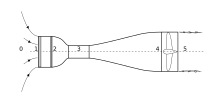
\includegraphics[width=0.90\textwidth]{./fig/wt}
\end{figure}

\sol

\partone
Si studia la galleria a circuito aperto rappresentata in figura utilizzando i bilanci integrali scritti per alcuni volumi di controllo fissi, per ricavare l'andamento della velocità e della pressione all'interno della galleria e infine ricavare la potenza dei motori, necessaria per garantire le condizioni di progetto nella sezione di prova. Si ipotizza un funzionamento stazionario, si trascurano gli effetti viscosi nel volume e sulle pareti della galleria e le forze di volume. In particolare, grazie alle ipotesi fatte, si possono semplificare il bilancio di massa,
\begin{equation}
\begin{aligned}
 & \dfrac{d}{dt} \int_V \rho = - \oint_{S} \rho \bm{u} \cdot \bm{\hat{n}} 
 \hspace{1.0cm} \rightarrow \hspace{1.0cm} \oint_{S} \rho \bm{u} \cdot \bm{\hat{n}} = 0 \ ,
\end{aligned}
\end{equation}
e il bilancio dell'energia cinetica,
\begin{equation}
\begin{aligned}
 & \dfrac{d}{dt} \int_V \rho \dfrac{|\bm{u}|^2}{2} = - \oint_{S} \rho \dfrac{|\bm{u}|^2}{2} \bm{u} \cdot \bm{\hat{n}} + \oint_S \bm{t_n} \cdot \bm{u} - \int_V \bm{\nabla} \bm{u} : \mathbb{T} + \int_V \rho \bm{g} \\
 & \hspace{1.0cm} \rightarrow \hspace{1.0cm} 
 - \oint_{S} \rho \dfrac{|\bm{u}|^2}{2} \bm{u} \cdot \bm{\hat{n}} + \oint_S \bm{t_n} \cdot \bm{u} = 0 \ . 
\end{aligned}
\end{equation}

\parttwo
Viene svolta la prima parte dell'esercizio, trascurando le perdite di pressione che avvengono tra la sezione 1 e la sezione 2, a causa della presenza dei nidi d'ape e delle reti.
\newline \noindent
Si scrive il bilancio di massa per un volume di fluido che ha come superficie di contorno la superficie $S_0$, la superficie laterale del tubo di flusso e una superficie $S_i$ all'interno della galleria. Assumendo grandezze uniformi sulla sezione, si può scrivere
\begin{equation}
 \rho A_0 U_0 = \rho A_i U_i \ ,
\end{equation}
cioè che il flusso di massa $\dot{m}$ che attraversa le sezioni della galleria è costante. Se sono note le condizioni di progetto in camera di prova, da esser si può calcolare il flusso di massa,
\begin{equation}
 \dot{m} = \rho A_3 U_3 = \rho A_{test} V_{test} = \dots \ .
\end{equation}
Poiché la velocità all'infinito è nulla, $U_0 \rightarrow 0$, l'area della sezione all'infinito a monte deve tendere all'infinito $A_0 \rightarrow \infty$.
\newline \noindent
Si scrive poi il bilancio di energia cinetica per un volume di controllo che ha come contorno la superficie $S_0$ all'infinito a monte, dove viene aspirata l'aria in uno stato di quiete, la superficie laterale del tubo di flusso, la superficie interna della galleria e la sezione $S_4$ alla fine del divergente, poco prima dell'imbocco dei ventilatori. Poiché non ci sono organi meccanici in movimento, il termine $\oint_S \bm{t_n} \cdot \bm{u}$ è nullo, e assumendo grandezze fisiche costanti sulle sezioni si può scrivere,
\begin{equation}
 \rho A_0 U_0 \left( \dfrac{U_0^2}{2} + \dfrac{P_0}{\rho} \right) =
 \rho A_4 U_4 \left( \dfrac{U_4^2}{2} + \dfrac{P_4}{\rho} \right) \ .
\end{equation}
Poiché il flusso di massa che attraversa le sezioni considerate è costante, il bilancio di energia cinetica si riduce a un'espressione che ricorda quella del teorema di Bernoulli, così come viene enunciato alle scuole superiori,
\begin{equation}
 P_0 + \dfrac{1}{2} \rho \, U_0^2  = P_4 + \dfrac{1}{2} \rho \, U_4^2
 \qquad \rightarrow \qquad B_4 = B_0 = P_{atm} \ ,
\end{equation}
avendo introdotto la definizione del ``binomio di Bernoulli'', $B_i = P_i + \rho U_i^2 / 2$.
\newline \noindent
Si scrive poi il bilancio di energia cinetica per il volume fluido $V(t)$ che contiene il ventilatore, delimintato dalle superifci $S_4$, $S_5$ e la superficie interna della galleria e dalla superficie (mobile!) del ventilatore. Il bilancio diventa
\begin{equation}
\int_{S_4} \rho \dfrac{|\bm{u}|^2}{2} \bm{u} \cdot \bm{\hat{n}} - \bm{t_n} \cdot \bm{u} + 
\int_{S_5} \rho \dfrac{|\bm{u}|^2}{2} \bm{u} \cdot \bm{\hat{n}} - \bm{t_n} \cdot \bm{u} = \int_{S_{fan}} \bm{t_n} \cdot \bm{u} \ ,
\end{equation}
essendo il termine a destra dell'uguale la potenza delle forze essercitata dal ventilatore sul fluido, contraria a quella esercitata dal fluido sul ventilatore, ma uguale a quella che deve fornire il motore elettrico per poter garantire la rotazione del ventialore stesso. Se si trascurano gli sforzi viscosi sulle superfici $S_4$ ed $S_5$, $\bm{t_n} = \bm{s_n} - P \bm{\hat{n}}$, e se si esplicita la potenza che deve essere fornita dai motori, il bilancio diventa,
\begin{equation}
 W_{mot} = 
\int_{S_4} \left( \rho \dfrac{|\bm{u}|^2}{2} + P \right) \left( \bm{u} \cdot \bm{\hat{n}} \right)  + 
\int_{S_5} \left( \rho \dfrac{|\bm{u}|^2}{2} + P \right) \left( \bm{u} \cdot \bm{\hat{n}} \right) \ , 
\end{equation}
e facendo l'ipotesi di grandezze fisiche costanti sulle sezioni,
\begin{equation}
 W_{mot} = \rho A_5 U_5 \left( \dfrac{U_5^2}{2} + \dfrac{P_5}{\rho} \right) 
         - \rho A_4 U_4 \left( \dfrac{U_4^2}{2} + \dfrac{P_4}{\rho} \right)
         = \dot{m} \left( B_5 - B_4 \right) \ . 
\end{equation}
Ricordando che il ``binomio di Bernoulli'' nelle sezioni 1:4 è uguale al ``binomio di Bernoulli'' nella sezione $S_0$, e quindi uguale alla pressione ambiente $P_{atm}$, nell'ipotesi che la pressione nella sezione $S_5$ sia uguale alla pressione atmosferica $P_{atm}$ all'esterno del tubo di flusso, la potenza del motore diventa,
\begin{equation}
 W_{mot} = \dot{m} \dfrac{U_5^2}{2} \ ,
\end{equation}
e, riferendosi alle grandezze fisiche in camera di prova, può essere scritta come
\begin{equation}
\begin{aligned}
 & W_{mot} = \dot{m} \left( \dfrac{A_{test}}{A_{fan}} \right)^2 \dfrac{V_{test}^2}{2} \\
 & \hspace{3.0cm} \rightarrow \qquad 
 W_{mot} = \dfrac{1}{2} \rho A_{test} \left( \dfrac{A_{test}}{A_{fan}} \right)^2 V_{test}^3 = \dots kW \ .
\end{aligned}
\end{equation}
La formula della potenza dei motori necessaria al funzionamento della galleria mette in evidenza la dipendenza dal cubo della velocità di prova e dal quadrato del rapporto tra l'area della sezione di prova e l'area della sezione all'imbocco delle ventole. Questo ultimo termine dovrebbe chiarire uno degli obiettivi del divergente della galleria: rallentare la corrente dopo la sezione di prova, per poter ridurre la potenza dei motori da installare per garantire il funzionamento dell'impianto.
%
\newline \noindent
\textbf{Osservazione.} Potrebbe suscitare qualche perplessità il fatto che la corrente in uscita dall'impianto con velocità $U_5 \simeq V_{fan}$ abbia una pressione uguale alla pressione ambiente, $P_{atm}$, come il fluido in quiete all'esterno del tubo di flusso. {\color{red} Provando ad applicare il teorema di Bernoulli} tra un punto sulla sezione del tubo di flusso $S_5$ e un punto all'esterno del tubo di flusso,
{\color{red}
\begin{equation}
 P_5 + \dfrac{1}{2}\rho V_{fan}^2 = P_5^{out}
 \quad \rightarrow \quad 
 P_{atm} + \dfrac{1}{2}\rho V_{fan}^2 = P_{atm} \ ,
\end{equation}
}
si giungerebbe alla conclusione che {\color{red} $V_{fan} = 0$}. L'errore risiede nell'applicazione del teorema di Bernoulli nella formula vista alla scuola superiore (o in altri corsi universitari), nonostante alcune ipotesi (che verranno presentate nel prosieguo del corso) non siano rispettate. In particolare, per collegare un punto sulla sezione $S_5$ e un punto all'esterno del tubo di flusso viene attraversato uno strato di mescolamento tra la corrente in moto che esce dalla galleria e il fluido in quiete all'esterno: la presenza di questo strato di mescolamento, nel quale la corrente non è irrotazionale $\bm{\omega} \neq 0$, fa cadere le ipotesi del teorema di Bernoulli e lo rende quindi inapplicabile. Tutte {\color{red}le parti evidenziate in rosso devono quindi essere considerate errate}.
